\documentclass[11pt]{scrartcl}
\usepackage{graphicx}
\graphicspath{{./}}
\usepackage[sexy]{evan}
\usepackage[normalem]{ulem}
\usepackage{hyperref}
\usepackage{mathtools}
\hypersetup{
    colorlinks=true,
    linkcolor=blue,
    filecolor=magenta,      
    urlcolor=cyan,
    pdfpagemode=FullScreen,
    }

\renewcommand{\dangle}{\measuredangle}

\renewcommand{\baselinestretch}{1.5}

\addtolength{\oddsidemargin}{-0.4in}
\addtolength{\evensidemargin}{-0.4in}
\addtolength{\textwidth}{0.8in}
% \addtolength{\topmargin}{-0.2in}
% \addtolength{\textheight}{1in} 


\setlength{\parindent}{0pt}

\usepackage{pgfplots}
\pgfplotsset{compat=1.15}
\usepackage{mathrsfs}
\usetikzlibrary{arrows}

\title{G7-8}
\author{Azzam Labib (IG: haxuv.world)}
\date{\today}
\begin{document}
\maketitle
\section{Problems}
\begin{enumerate}
\item Evaluate
    $$15120 \times \left(\dfrac{2}{1 \times 2 \times 3} + \dfrac{3}{1 \times 2 \times 3 \times 4}+\dots+\dfrac{6}{1\times 2 \times 3 \times \ldots \times 7} \right)$$

\item In the equation below, $a$, $b$ and $c$ are digits, $\overline{aa}$ and $\overline{bb}$ are two-digit numbers, and $\overline{cccc}$ is a four-digit number.
\[\overline{aa}^2 + \overline{bb} = \overline{cccc}\]
What is the largest possible value of $a + b + c$?

\item The number 2019 is the smallest positive integer that can be written in 6 ways as the sum of squares of 3 prime numbers. One such way is:
\[x^2 + x^2 + 41^2 = 2019\]
What is the value of $x$?

\item What is the smallest four-digit number that is divisible by 1, 2, 3, 4, 5, 6, 7, 8, 9 and 10?

\item In the triangle below, $AB = BD = DE = EC$. Given $\angle ABE = 120^\circ$, what is the measure of $\angle BDA$?
\begin{figure}[h]
    \centering
    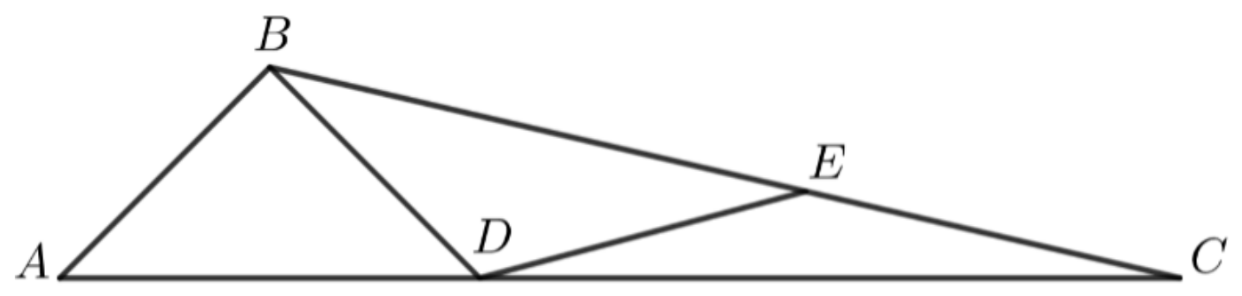
\includegraphics[scale=0.5]{Test For Pelatihan/triangle.png}
\end{figure}

\item Find the smallest positive integer $n$ for which $225n$ is a multiple of 4500.

\item Find the sum of the digits of the following product.
\[3\ldots 3 \times 2019\]
where the first term is a 100-digit number with all digits being 3.

\item In the rectangle ABCD, point E is on the side AB while point F in on the side AD such that $BE = \frac{1}{4}AE$ and $DF = \frac{2}{3}AD$. What is the ratio of areas of the rectangle ABCD to triangle FEC?
\begin{figure}[h]
    \centering
    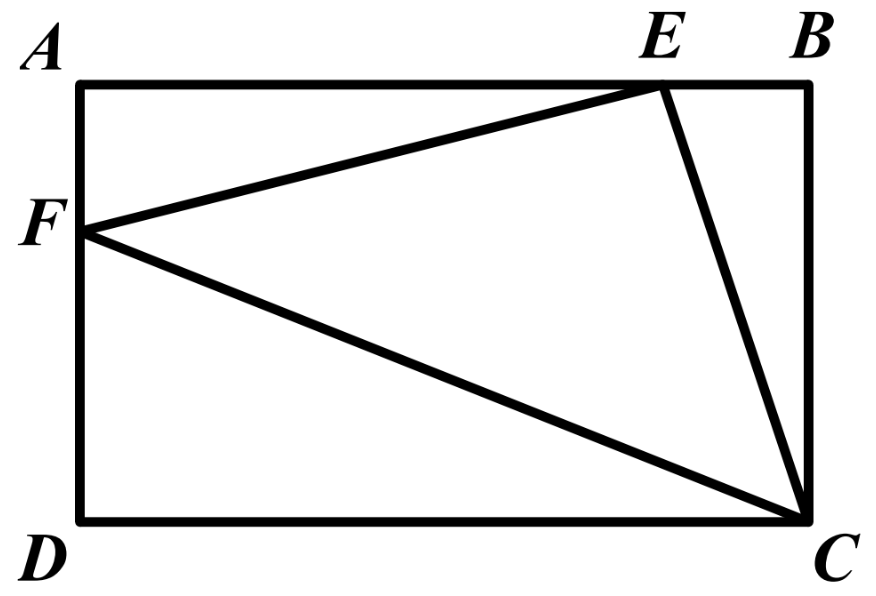
\includegraphics[scale=0.4]{Test For Pelatihan/rectangle.png}
\end{figure}

\item The six-digit number $2X475Y$ is divisible by 36. How many possible values of $X$ are there?

\item How many four-digit numbers are there between 3700 and 9600 that can be formed using only the digits 3, 7, 5, 6, 0 or 9 without repetition of any digits?

\item Find the value of 
\[\left[\sqrt{1 + 2 + 3 + \ldots + 100}\right],\]
where $[x]$ is the greatest integer less than or equal to $x$. For example, $[13.54] = 13$.

\item The operator $\otimes$ acts on two numbers to give the following outcomes:
\[2 \otimes 6 = 44\]
\[4 \otimes 10 = 87\]
\[8 \otimes 18 = 1613\]
\[16 \otimes 22 = 2019\]
Find the value of $7 \otimes 9$.

\item In a camp, 134 students received a burger and 62 received an ice cream. Fifteen students received burger and ice cream but not fries, and 31 students received all the three types of food. Given there are 200 students in this camp, what is the largest possible number of students who didn’t get any of the three types of food?
\end{enumerate}

\end{document}